\chapter{Conclusions and Discussion}\label{final}
 The present study involved exploring several deep learning models for handwritten character recognition using a dataset of hand-written characters in the form of images. The models used for this purpose included LSTM+CNN, CNN, and CNN+GRU, which were trained by hyper-tuning their parameters.
 
 Initially, a CNN model was trained on 26 small and 26 capital letters, achieving an accuracy of 98 percent for capital letters and 97 percent for small letters. This outcome demonstrated the ability of the CNN model to accurately recognize handwritten characters.

Subsequently, the CNN model was trained on all 52 classes, achieving an accuracy of 97.01 percent. This result indicates that the CNN model is capable of recognizing a broader range of handwritten characters with high precision.

The CNN+GRU model was then trained, and an accuracy of 97.61 percent was achieved. This outcome suggests that the addition of a GRU layer can potentially enhance the model's performance.

Finally, the LSTM+CNN model was trained and achieved an accuracy of 97.64 percent. This outcome represents the highest accuracy among all models tested and suggests that the incorporation of a recurrent layer, such as LSTM, can enable better capturing of long-term dependencies in the data.

In conclusion, the present study demonstrated the successful implementation of various deep learning models for handwritten character recognition using a dataset of hand-written characters in image format. The obtained results indicate that the incorporation of recurrent layers, such as LSTM and GRU, can enhance the performance of CNN models for this purpose.

\begin{figure}[htp]
    \centering
    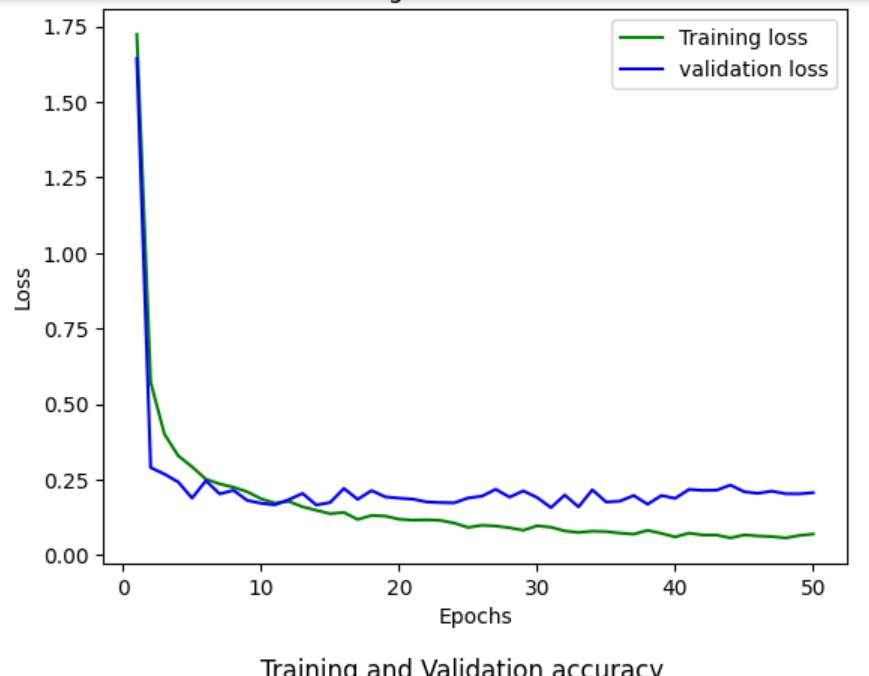
\includegraphics[width=8cm]{report/image1.png}
    \caption{The training and validation loss obtained from running a CNN model for 50 epochs}
    \label{fig:galaxy}
\end{figure}

\begin{figure}[htp]
    \centering
    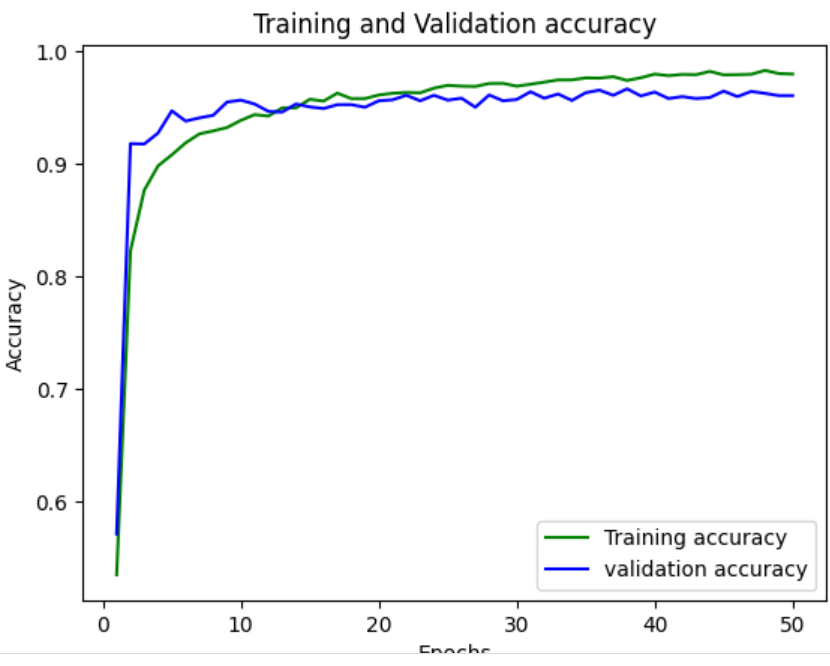
\includegraphics[width=8cm]{report/image2.png}
    \caption{The training and validation accuracy obtained from running a CNN model for 50 epochs}
    \label{fig:galaxy}
\end{figure}


\begin{center}
\begin{tabular}{||c c||} 
\hline
 Model & Accuarcy \\ [0.5ex] 
 \hline\hline
 CNN &  97.01  \\ 
 \hline
 ConvoGRU & 97.61 \\
 \hline
 CNN+LSTM & 97.64 \\ [1ex] 
\hline
\end{tabular}
\end{center}
\begin{center}
\caption{Table showing the accuracy of three different models }
\end{center}